\documentclass[conference]{IEEEtran}
\usepackage{amsmath,amssymb,booktabs,graphicx,url,multirow,array,xcolor}
\usepackage{tikz}
\usetikzlibrary{positioning,arrows.meta,fit,backgrounds}
\usepackage[hidelinks]{hyperref}
\graphicspath{{figs/}}

% ---- Submission switch: IJCNN 2027 uses double-blind review. \blindtrue for submission, \blindfalse for the final version.
\newif\ifblind
\blindtrue
\newcommand{\codeurl}{\ifblind an anonymised repository (link withheld for review)\else\url{https://github.com/sidddha2004/drift-detection}\fi}
\newcommand{\fone}{macro-F1}
\newcommand{\tla}{TLA}

\begin{document}

\title{When Does Drift Typing Help? A Pre-Registered Study of Local Adaptation in Federated Wearable HAR}

\ifblind
\author{\IEEEauthorblockN{Anonymous Authors}\IEEEauthorblockA{Paper under double-blind review}}
\else
\author{
\IEEEauthorblockN{Abhinav Agrawal, Siddharth Solanki}
\IEEEauthorblockA{Dept. of Computer Science and Engineering\\
The LNM Institute of Information Technology, Jaipur, India\\
\{23ucs506, 23ucs714\}@lnmiit.ac.in}
\and
\IEEEauthorblockN{Richa Priyadarshani}
\IEEEauthorblockA{Dept. of Communication and Computer Engineering\\
The LNM Institute of Information Technology, Jaipur, India\\
richa.priyadarshani@lnmiit.ac.in}
}
\fi

\maketitle

\begin{abstract}
Federated models for wearable human activity recognition (HAR) lose accuracy when a sensor rotates, its gain changes, or an activity label changes meaning after deployment. A tempting remedy is to detect the drift on the device, guess its type, and apply a cheap repair matched to that type. We test this idea carefully rather than promote it. On a PAMAP2 benchmark with ground-truth drift events (8 clients; sudden, gradual, recurring and sensor-level drift) and a pre-registered analysis over 10 held-out seeds, we compare typed local adaptation (\tla{}) with no adaptation, fixed local repairs and federated retraining. Four findings stand out. (i) Uploading only a 1{,}966-parameter adapter instead of the full model cuts uplink by 96\% with no loss in accuracy; most of this saving follows directly from the adapter's size. (ii) Local adaptation leaves clients that did not drift untouched, whereas periodic federated retraining lowers their \fone{} by about 5 points. (iii) Typing does not beat simply retraining the classifier head after every alarm, and on recurring drift \tla{} is worse than no adaptation, because responses arrive late and are never undone. (iv) Guessing the type wrong is costly: aligning the input against a label change loses up to 0.21 \fone{}. Both the detector and the repairs need labels on the device; only the type classifier is label-free.
\end{abstract}

\begin{IEEEkeywords}
federated learning, concept drift, human activity recognition, wearable sensors, on-device adaptation
\end{IEEEkeywords}

% =====================================================================
\section{Introduction}
Federated learning (FL) lets wearable devices train a shared activity model without sending raw data~\cite{mcmahan2017fedavg,aouedi2024fedhar}. After deployment, however, the data drift~\cite{gama2014survey,lu2019learning}: a strap slips and rotates the sensor axes, a replacement sensor has a different gain, or an application redefines an activity. Drift comes in two kinds. Under \emph{virtual} drift the input distribution $P(X)$ changes and $P(Y\mid X)$ stays fixed, so the fault can be undone at the input. Under \emph{real} drift $P(Y\mid X)$ changes, so the classifier itself must change. Most federated drift methods treat both alike and retrain the full model~\cite{jothimurugesan2023feddrift,panchal2023flash}, which costs megabytes of uplink per episode.

This suggests an appealing design: detect drift on the device, \emph{type} it as virtual or real, and apply a cheap local repair matched to the type. This paper asks when that design actually helps. We test it under a pre-registered protocol and report where it works and where it fails.

\textbf{Labels are required.} Every system studied here, ours included, needs correct labels on the device soon after the data arrive: the drift detector monitors the model's errors, and both repairs fit to labelled windows. Only the type classifier works without labels. Our results therefore apply to settings with prompt, if sparse, labels (here about two labelled windows per client and round), for example through user confirmation or self-labelling apps.

\textbf{Contributions.} In order of importance:
\begin{enumerate}
\item \emph{Adapter-only federation.} Sending a small adapter instead of the whole model cuts uplink by 96\% with no loss in post-change \fone{} (a pre-registered non-inferiority test). This mostly reflects the adapter's size (1{,}966 vs.\ 53{,}260 parameters, 3.7\%): the finding is that the small adapter is \emph{enough}, not that it compresses anything.
\item \emph{Protection of clean users.} Local adaptation leaves clients that did not drift unchanged, whereas periodic federated retraining lowers their \fone{} by about 5 points.
\item \emph{A diagnosed failure.} Typed adaptation fails on recurring drift; we show that half of its responses arrive after the drift has ended and are never undone, and that a cached-state memory cannot fix this with sparse labels.
\item \emph{The cost of a wrong type.} Applying the virtual-drift repair to a real drift loses 0.18--0.21 \fone{}; the costs of type errors are asymmetric.
\end{enumerate}
We also release a PAMAP2 drift benchmark with a ground-truth change-point manifest and a streaming simulator that counts every transmitted byte. Typed adaptation does \emph{not} outperform a fixed head-retraining response (H5 fails), and we make no claim that it does.

% =====================================================================
\section{Related Work}
\textbf{FL under drift.} FedDrift detects drift per client and clusters clients into concept-specific models~\cite{jothimurugesan2023feddrift}; Flash adapts client and server learning rates when drift occurs~\cite{panchal2023flash}; FedConD handles asynchronous sensor clients~\cite{chen2021fedcond}; CDA-FedAvg combines local detection with rehearsal on HAR data~\cite{casado2022cdafedavg}; FedStream tracks streams with class prototypes~\cite{mawuli2023fedstream}; Chen~\emph{et al.} adapt to virtual drift separately from real drift~\cite{chen2025virtual}; a recent survey organises the field by temporal profile, coverage and synchrony~\cite{mahdi2025fdal}. \emph{Difference:} these methods aggregate model updates after drift; we measure how far a client gets with zero-uplink repairs, and count the bytes of every alternative.

\textbf{Memory for recurring concepts.} Stream learners reuse models when an old concept returns: Katakis~\emph{et al.} cluster batches into contexts and keep an ensemble per context~\cite{katakis2010recurring}; RCD stores a classifier and a data sample per context and reuses it when a multivariate test matches the new data~\cite{goncalves2013rcd}; Gama and Kosina learn meta-models that predict which stored model applies~\cite{gama2014recurrent}. \emph{Difference:} these methods see far more labelled data per decision than a wearable client; we show that with about two labels per round, error-based reuse cannot tell when a concept has returned.

\textbf{HAR under sensor displacement.} Displacement and rotation of body-worn sensors are a known cause of accuracy loss~\cite{kunze2014placement,banos2014displacement}. Remedies include robust sensor fusion~\cite{banos2014displacement} and unsupervised recalibration that estimates the shift in feature space~\cite{chavarriaga2013unsupervised}. \emph{Difference:} we treat displacement as one drift type inside a federated stream, fix it with a closed-form input map, and test whether choosing between repairs by drift type pays off.

% =====================================================================
\section{Benchmark, Method and Protocol}
\textbf{Data and model.} We use PAMAP2~\cite{reiss2012pamap2} subjects 101--108 as 8 clients (subject 109 has one 64\,s bout and is excluded), the nine $\pm16$\,g accelerometer channels of the hand, chest and ankle IMUs, and windows of 256 samples (stride 128) cut inside activity bouts after trimming 5\,s at each end. Contiguous 16-window blocks form train/validation/test splits (60/15/25\%) with a purge between splits, and normalisation uses frozen training statistics. The classifier is a \emph{two-layer} LSTM with 64 hidden units and a 12-way head: $19{,}200+33{,}280$ LSTM weights plus $780$ head weights, i.e., 53{,}260 parameters (208\,kB). All systems start from the same personalised model (FedAvg for 60 rounds, then local fine-tuning; clean \fone{} 0.935).

\textbf{Drift.} Virtual drift adds a 1\,g offset, a $\times1.3$ gain or a $20^\circ$ rotation to the raw signal; real drift swaps the labels of two class pairs. Streams have 120 rounds, about two labelled windows per client and round (median 2, range 1--3), and 3 of 8 clients drift. Scenarios: \textbf{S1} sudden onset at round 30 (gain, rotation, offset, real); \textbf{S2} 10-round ramp with onsets in rounds 30--40 (rotation, real); \textbf{S3} recurring, drift on in rounds 30--44, 60--74, 90--104 (rotation, real); \textbf{S4} one sensor only (ankle gain, chest rotation); \textbf{S0} no drift (control). The primary endpoint is the \emph{post-change \fone{}} of the drifted clients from onset to the end of the stream.

\textbf{Typed local adaptation (\tla{}).} Fig.~\ref{fig:system} shows the pipeline. Each client runs a Page--Hinkley test~\cite{page1954} on its error bit ($\delta=0.05$, $\lambda=8$, tuned on tuning seeds under one false alarm per 1{,}000 clean windows). Five rounds after an alarm, a gradient-boosting classifier~\cite{friedman2001gbm} predicts virtual or real drift from \emph{label-free} features (changes of window statistics, prediction entropy and per-sensor shift). Virtual drift is repaired by a closed-form, ridge-regularised affine map per IMU that moves the class means of recent drifted windows onto stored clean class means; it is written into a 90-parameter input layer and needs no gradient step. Real drift is repaired by retraining the 780-parameter head on the last 45 rounds of labelled windows, replaying clean windows of classes missing from that buffer. \tla{} uploads nothing.

\begin{figure}[t]
\centering
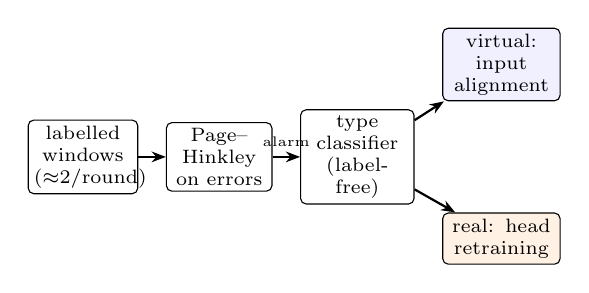
\begin{tikzpicture}[node distance=3mm and 3.5mm,
  box/.style={draw, rounded corners=2pt, align=center, font=\scriptsize, minimum height=6.5mm, inner sep=2pt},
  arr/.style={-{Stealth[length=1.8mm]}, thick}]
\node[box, text width=1.25cm] (s) {labelled windows ($\approx$2/round)};
\node[box, text width=1.2cm, right=of s] (ph) {Page--Hinkley on errors};
\node[box, text width=1.3cm, right=of ph] (ty) {type classifier (label-free)};
\node[box, text width=1.35cm, above right=1mm and 3.5mm of ty, fill=blue!6] (al) {virtual: input alignment};
\node[box, text width=1.35cm, below right=1mm and 3.5mm of ty, fill=orange!10] (hd) {real: head retraining};
\draw[arr] (s) -- (ph); \draw[arr] (ph) -- node[above, font=\tiny]{alarm} (ty);
\draw[arr] (ty) -- (al); \draw[arr] (ty) -- (hd);
\end{tikzpicture}
\caption{Typed local adaptation on one client. Detection and both repairs use labels; only the type classifier does not. Nothing is uploaded.}
\label{fig:system}
\end{figure}

\textbf{Systems compared.} No adaptation: \emph{Global} (FedAvg model) and \emph{Personalized} (the shared starting model). Federated retraining of the full model: \emph{Periodic} (every 10 rounds), \emph{ADWIN + full} and \emph{PH + full} (after an ADWIN~\cite{bifet2007adwin} or Page--Hinkley alarm), and \emph{PH + FedProx} (with a proximal term, $\mu=1$~\cite{li2020fedprox}). \emph{PH + federated adapter}: alarmed clients train and average the adapter, i.e., the input layer (90), a rank-8 residual bottleneck (1{,}096) and the head (780), 1{,}966 parameters or 7.9\,kB per upload. Local repairs: \emph{PH + local full retraining}, \emph{Input alignment (fixed)} and \emph{Head retraining (fixed)}, which apply one repair after every alarm, and \tla{}. Upper references: \tla{} with the true type, and oracle 2-way and 4-way typing with true alarm times. The federated baselines re-implement the response step of drift-aware FL on our backbone and are not the official code of FedDrift or FedProx.

\textbf{Protocol.} The analysis plan was committed before any evaluation run. Five hypotheses: \tla{} beats Personalized (H1), Periodic (H2) and PH + FedProx (H3); the federated adapter is non-inferior to PH + full within 0.010 \fone{} (H4); and \tla{} beats Head retraining (fixed), the best fixed response (H5). The unit of analysis is the seed; 10 evaluation seeds (7, 11, 13, 17, 19, 23, 42, 123, 999, 2024) are disjoint from the tuning seeds (1001--1010). Each test is a paired two-sided Wilcoxon signed-rank test~\cite{wilcoxon1945}, with Holm correction~\cite{holm1979} over the 12 tests of H1--H3 and H5 on S1--S3, and a bootstrap 95\% CI as a secondary summary. With 10 seeds the smallest possible two-sided Wilcoxon $p$ is $2/2^{10}=0.00195$, so the smallest possible Holm-corrected $p$ over 12 tests is $0.0234$. We treat the Holm-corrected $p$-values as the primary evidence: the CI and the test can disagree (H2). The confirmatory run comprises 14 systems $\times$ 10 drift variants (4 in S1 and 2 each in S2--S4) $\times$ 10 seeds $=1{,}400$ streams. \emph{Disclosures:} tuning seeds 1004--1010 were viewed before some design changes; the comparators of H3 and H5 were chosen after tuning results were seen; the benchmark was lengthened once, before any evaluation run; the memory, S0 and privacy studies were added afterwards and are descriptive (S0: 7 systems $\times$ 10 seeds; memory: 2 configurations $\times$ 2 S3 variants $\times$ 10 seeds).

% =====================================================================
\section{Results}

\begin{table*}[t]
\centering
\caption{Post-change \fone{} of drifted clients (mean $\pm$ std over 10 seeds), \fone{} of clean clients under S1, and uplink per S1 run (kB $=1{,}000$ bytes). Bold: best non-reference system per column.}\label{tab:all}
\small
\setlength{\tabcolsep}{4.5pt}
\begin{tabular}{lcccccr}
\toprule
System & S1 sudden & S2 gradual & S3 recurring & S4 one sensor & Clean users (S1) & Uplink S1 \\
\midrule
Global (no adaptation) & $0.658\pm0.023$ & $0.590\pm0.029$ & $0.737\pm0.016$ & $0.635\pm0.030$ & -- & 0 \\
Personalized (no adaptation) & $0.677\pm0.022$ & $0.612\pm0.031$ & $0.761\pm0.019$ & $0.681\pm0.034$ & \textbf{0.944} & 0 \\
Periodic full retraining & $0.710\pm0.026$ & $0.635\pm0.021$ & $0.744\pm0.020$ & $0.726\pm0.024$ & 0.895 & 18{,}748 \\
ADWIN + full retraining & $0.699\pm0.021$ & $0.642\pm0.022$ & $0.733\pm0.021$ & $0.726\pm0.039$ & 0.943 & 2{,}269 \\
PH + full retraining & $0.704\pm0.015$ & $0.647\pm0.027$ & $0.735\pm0.014$ & $0.721\pm0.027$ & 0.940 & 3{,}387 \\
PH + FedProx retraining & $0.738\pm0.014$ & $0.669\pm0.019$ & $0.763\pm0.010$ & $0.761\pm0.024$ & 0.942 & 3{,}174 \\
PH + federated adapter & $0.710\pm0.021$ & $0.649\pm0.023$ & $0.746\pm0.016$ & $0.726\pm0.022$ & 0.940 & 127 \\
PH + local full retraining & $0.704\pm0.022$ & $0.647\pm0.029$ & $0.725\pm0.015$ & $0.722\pm0.035$ & -- & 0 \\
Input alignment (fixed) & $0.707\pm0.027$ & $0.616\pm0.051$ & $0.637\pm0.021$ & $\mathbf{0.820}\pm0.043$ & -- & 0 \\
Head retraining (fixed) & $0.753\pm0.022$ & $\mathbf{0.707}\pm0.027$ & $\mathbf{0.766}\pm0.014$ & $0.753\pm0.019$ & 0.942 & 0 \\
\tla{} (typed) & $\mathbf{0.756}\pm0.050$ & $0.691\pm0.077$ & $0.711\pm0.051$ & $0.810\pm0.044$ & 0.943 & 0 \\
\tla{} + memory (descriptive) & -- & -- & $0.709\pm0.059$ & -- & -- & 0 \\
\midrule
\tla{} with true type & $0.783\pm0.028$ & $0.744\pm0.029$ & $0.734\pm0.019$ & $0.819\pm0.041$ & -- & 0 \\
Oracle 2-way typing$^{\dagger}$ & $0.779\pm0.049$ & $0.717\pm0.035$ & $0.731\pm0.020$ & $0.811\pm0.061$ & -- & 0 \\
Oracle 4-way typing$^{\dagger}$ & $0.779\pm0.049$ & $0.762\pm0.031$ & $0.797\pm0.018$ & $0.863\pm0.043$ & -- & 0 \\
\bottomrule
\multicolumn{7}{l}{\footnotesize $^{\dagger}$True alarm times and types. Oracle 2-way uses one-shot alignment without tracking, so it can score below \tla{} with the true type; these rows are references, not upper bounds.}
\end{tabular}
\end{table*}

\subsection{Adapter-only federation (H4)}
Uploading only the adapter is non-inferior to full-model retraining on every scenario (PH + full minus adapter: $-0.005$ $[-0.015,+0.005]$ on S1, $-0.002$ $[-0.013,+0.008]$ on S2, $-0.011$ $[-0.022,-0.000]$ on S3; every upper bound is below the $+0.010$ margin) and sends 96\% fewer bytes (127 vs.\ 3{,}387\,kB per S1 run, Table~\ref{tab:all}). The saving is close to the ratio of the payload sizes (3.7\%); the result is that this small payload loses nothing. Fig.~\ref{fig:cost} adds the local systems: Head retraining (fixed) and \tla{} reach equal or higher \fone{} than every federated system without any upload.

\begin{figure}[t]
\centering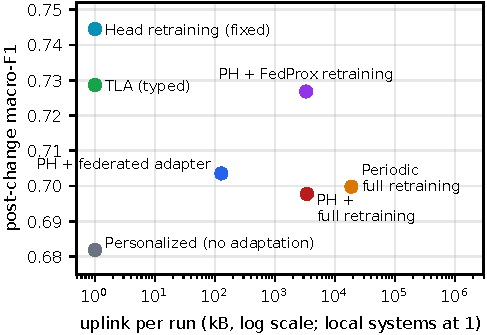
\includegraphics[width=\columnwidth]{cost_vs_uplink.pdf}
\caption{Accuracy against uplink, mean over S1--S3 and 10 seeds. Local systems (no upload) are drawn at 1\,kB.}
\label{fig:cost}
\end{figure}

\subsection{Clean users}
Federation spreads drift. Under S1, periodic federated retraining lowers the \fone{} of the five clients that did not drift from 0.944 to 0.895 (about 5 points; 4.4--5.4 across the drift variants), because drifted updates enter the shared model on a fixed schedule (Table~\ref{tab:all}). Alarm-triggered retraining averages fewer, later updates and costs 0.1--0.4 points; local repairs, including \tla{}, leave clean clients essentially unchanged (0.943).

\subsection{Typed adaptation against the baselines (H1--H3, H5)}
Table~\ref{tab:conf} gives the 12 confirmatory tests. \tla{} beats no adaptation on sudden drift (H1, S1: $+0.079$, Holm $p=0.023$, the smallest attainable value). On gradual drift the difference is the same size ($+0.080$) but not significant after correction ($p=0.078$), although its bootstrap CI excludes zero; we do not claim it. Against periodic retraining (H2) and PH + FedProx (H3), \tla{} is not significantly better on S1 or S2; it matches them without uplink. \textbf{H5 fails: \tla{} does not beat simply retraining the head after every alarm} (S1 $+0.004$, S2 $-0.016$, both $p=1.0$), and is significantly worse on recurring drift (S3, $-0.055$), where it also loses to no adaptation (H1, $-0.050$) and to PH + FedProx (H3, $-0.052$). Typing pays for its errors and its five-round delay: with the true type, \tla{} would gain $0.027$, $0.053$ and $0.023$ on S1--S3.

\begin{table}[t]
\centering
\caption{Confirmatory tests, \tla{} minus comparator (post-change \fone{}, 10 seeds). Primary evidence: Holm-corrected Wilcoxon $p$ (minimum attainable 0.023).}\label{tab:conf}
\small
\setlength{\tabcolsep}{3pt}
\begin{tabular}{llrcr}
\toprule
H, comparator & Scen. & Diff. & 95\% CI & Holm $p$ \\
\midrule
H1 Personalized & S1 & $+0.079$ & $[+0.055,+0.105]$ & \textbf{0.023} \\
 & S2 & $+0.080$ & $[+0.040,+0.120]$ & 0.078 \\
 & S3 & $-0.050$ & $[-0.074,-0.029]$ & \textbf{0.023} \\
H2 Periodic & S1 & $+0.046$ & $[+0.008,+0.085]$ & 0.633 \\
 & S2 & $+0.057$ & $[+0.003,+0.109]$ & 0.588 \\
 & S3 & $-0.033$ & $[-0.070,+0.002]$ & 0.967 \\
H3 PH + FedProx & S1 & $+0.018$ & $[-0.008,+0.047]$ & 1.000 \\
 & S2 & $+0.023$ & $[-0.021,+0.063]$ & 1.000 \\
 & S3 & $-0.052$ & $[-0.084,-0.025]$ & \textbf{0.035} \\
H5 Head (fixed) & S1 & $+0.004$ & $[-0.019,+0.026]$ & 1.000 \\
 & S2 & $-0.016$ & $[-0.054,+0.019]$ & 1.000 \\
 & S3 & $-0.055$ & $[-0.082,-0.031]$ & \textbf{0.023} \\
\bottomrule
\end{tabular}
\end{table}

\subsection{The cost of a wrong type}
The two repairs are not interchangeable (Fig.~\ref{fig:mistype}). Aligning the input against a real drift makes things worse than doing nothing: 0.40, 0.42 and 0.55 \fone{} on the real-drift variants of S1--S3, against 0.58, 0.60 and 0.76 without adaptation, a loss of 0.18--0.21. Retraining the head on a virtual drift is harmless but recovers less than alignment. The type classifier reaches 0.839 accuracy in leave-one-seed-out validation, but recalls only 72\% of real drifts, so its errors fall on the costly side. This asymmetry explains why the head-retraining default is so hard to beat.

\begin{figure}[t]
\centering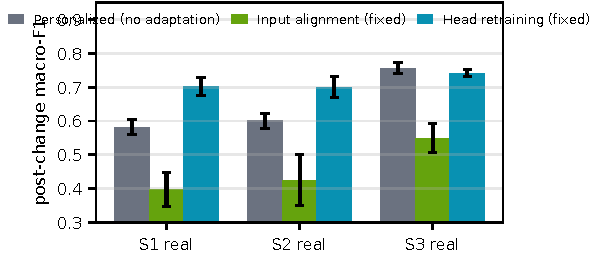
\includegraphics[width=\columnwidth]{mistype_cost.pdf}
\caption{Real-drift variants: input alignment, the virtual-drift repair, is worse than no adaptation; head retraining recovers accuracy (mean $\pm$ std over seeds).}
\label{fig:mistype}
\end{figure}

\subsection{Recurring drift: why typing fails, and a memory that does not help}
Splitting S3 into drift-on and drift-off phases locates the loss (Fig.~\ref{fig:recurring}). While the rotation is active, \tla{} beats no adaptation (0.692 vs.\ 0.598), but between episodes it falls far below it (0.780 vs.\ 0.932). Two mechanisms cause this. The repair is never undone, so the input map fitted to the rotated signal is applied to clean signals; and with a median detection delay of 23 rounds plus the typing delay, 18 of 36 responses start after the 15-round episode has ended.

\textbf{A memory does not fix it.} We gave each client a memory of $K$ cached adapter states. At each alarm the candidates (the original model, the current state and the cached states) are scored by their error on recent labelled windows, and the client switches to the best one if its error is within a tolerance of its normal error; otherwise \tla{} runs and caches the result. The configuration was selected on tuning seeds by a pre-registered rule ($K=0$, i.e., undo only; tolerance 0.02) and then run on S3 with all 10 evaluation seeds. It switched only 8 times in 20 S3 streams, and changed neither the post-change \fone{} ($0.709$ vs.\ $0.711$; difference $-0.002$ $[-0.011,+0.003]$, Wilcoxon $p=0.38$) nor the \fone{} between episodes ($0.785$ vs.\ $0.784$, $p=0.38$); a larger memory ($K=4$) gave identical results (Table~\ref{tab:all}, Fig.~\ref{fig:recurring}). The cause is statistical. On tuning seeds, scoring on windows since the alarm never undid (0 of 13 responses that started after the drift ended), because that window lies inside the drift episode; scoring on the last three rounds undid correctly 7 times but wrongly 6 times, because three rounds hold only about six labelled windows from one or two activities. \emph{With about two labelled windows per round, an error-based rule cannot tell drift-on from drift-off within a few rounds}, the same limit that delays detection. Reuse methods from stream mining~\cite{katakis2010recurring,goncalves2013rcd,gama2014recurrent} assume far more labels per decision; a label-free signature of the drift regime is the natural next step.

\begin{figure}[t]
\centering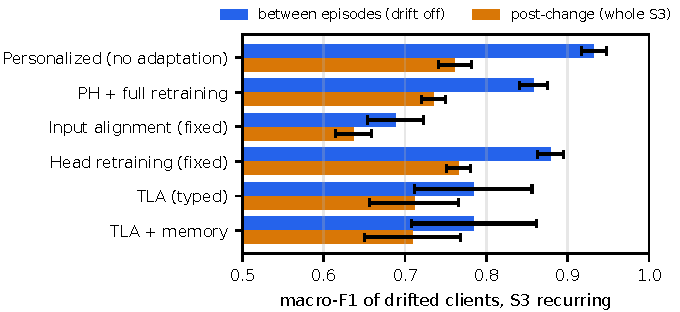
\includegraphics[width=\columnwidth]{recurring.pdf}
\caption{S3 recurring drift: \fone{} of drifted clients between episodes (drift off) and over the whole post-change period (mean $\pm$ std over seeds). Systems that keep their adaptation fall below no adaptation once the drift is gone.}
\label{fig:recurring}
\end{figure}

\subsection{No drift (S0)}
With no drift at all (S0, 10 evaluation seeds), the Page--Hinkley detector raised 0.9--1.5 false alarms per 8-client, 120-round stream, consistent with the validation rate of about 0.5 per 1{,}000 labelled windows. The repairs triggered by these false alarms barely cost accuracy: whole-stream \fone{} falls by 0.1 points for \tla{} and Head retraining (fixed) and by 0.3--0.5 points for input alignment, the federated adapter and PH + full retraining, against 0.939 with no adaptation. Periodic federated retraining, which does not wait for an alarm, loses 4.1 points ($0.899$) and uploads 18.7\,MB although nothing has changed.

\subsection{Device memory and privacy of uploads}
Per client in FP32, the model takes 208\,KiB, the adapter and each cached state 7.7\,KiB, but the replay pool dominates (8.5\,MiB for the median client), giving a peak of 9.0--9.5\,MiB for every adapting system. For the federated systems we also tested client-level differential privacy on uploads~\cite{mcmahan2018dpfl}: clipping to the median update norm and adding Gaussian noise with multiplier $z\in\{0.5,1,2,4\}$ ($\varepsilon\approx55$ to 4 per client, $\delta=10^{-5}$, R\'enyi accountant~\cite{mironov2017rdp}; 640 runs). Every noisy setting drops \fone{} from 0.70 to about 0.27, below no adaptation (Fig.~\ref{fig:dp}). The cause is dimensional: noise of norm $zC\sqrt d$ ($22C$ for the adapter at $z=0.5$) cannot be averaged down by $\sqrt 8$ clients. At this cohort size, keeping updates on the device is the only option we tested that keeps both accuracy and an unspent privacy budget.

\begin{figure}[t]
\centering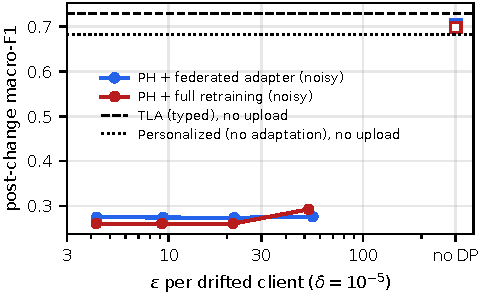
\includegraphics[width=\columnwidth]{dp_cliff.pdf}
\caption{Client-level DP on uploads (S1--S3, 10 seeds). Squares: no noise. Any noise leads to a cliff, not a trade-off.}
\label{fig:dp}
\end{figure}

% =====================================================================
\section{Limitations}
Both detection and repair need prompt labels on the device; with delayed labels the detection delay, already the main bottleneck (median 23 rounds), would grow. We use one dataset with injected, not natural, drift and 8 clients; severities were calibrated once; no official implementation of a drift-aware FL method was run; \tla{} varies more across seeds (std 0.05--0.08) than the baselines (about 0.02); run times and memory are measured in simulation, not on a wearable device.

\section{Conclusion}
Drift typing helps less than it seems. The robust gains in this study come from \emph{where} adaptation happens, not from typing: uploading only a small adapter keeps accuracy at 4\% of the bytes, and local repairs protect users who did not drift. A typed choice of repair does not beat a fixed head-retraining default, because wrong types are costly and typing adds delay, and it fails on recurring drift because sparse labels cannot reveal when a drift has ended. Faster label-efficient detection and a label-free signal for ``the drift is over'' are what typed adaptation needs next. Code, configurations and raw results: \codeurl.

\bibliographystyle{IEEEtran}
\bibliography{refs}

\end{document}
